\documentclass[a4paper,12pt]{article} 

% First, we usually want to set the margins of our document. For this we use the package geometry.
\usepackage[top = 2.5cm, bottom = 2.5cm, left = 2.5cm, right = 2.5cm]{geometry} 
\usepackage[T1]{fontenc}
\usepackage[utf8]{inputenc}

% The following two packages - multirow and booktabs - are needed to create nice looking tables.
\usepackage{multirow} % Multirow is for tables with multiple rows within one cell.
\usepackage{booktabs} % For even nicer tables.

% As we usually want to include some plots (.pdf files) we need a package for that.
\usepackage{graphicx} 

% The default setting of LaTeX is to indent new paragraphs. This is useful for articles. But not really nice for homework problem sets. The following command sets the indent to 0.
% \usepackage{setspace}
% \setlength{\parindent}{0in}
\usepackage{indentfirst}

% Package to place figures where you want them.
\usepackage{float}

% The fancyhdr package let's us create nice headers.
\usepackage{fancyhdr}

\usepackage{amsmath,amsthm}
\usepackage{minted}

\begin{document}

\section*{Practice 1: Control}

\subsection*{Code}

\begin{center}
    \begin{minted}{verilog}
module Controller(
input [6:0] Inst,
output reg Branch,
output reg [1:0] ALUOp,
output reg ALUSrc,
output reg MemRead,
output reg MemWrite,
output reg MemtoReg,
output reg RegWrite
    );
    
always @*
begin
    case(Inst)
        7'b0110011: // R-type
        begin
            Branch = 1'b0;
            ALUOp = 2'b10;
            ALUSrc = 1'b0;
            MemRead = 1'b0;
            MemWrite = 1'b0;
            MemtoReg = 1'b0;
            RegWrite = 1'b1;
        end
        7'b0010011: // I-type
        begin
            Branch = 1'b0;
            ALUOp = 2'b00;
            ALUSrc = 1'b1;
            MemRead = 1'b0;
            MemWrite = 1'b0;
            MemtoReg = 1'b0;
            RegWrite = 1'b1;
        end
        7'b0000011: // I-type
        begin
            Branch = 1'b0;
            ALUOp = 2'b00;
            ALUSrc = 1'b1;
            MemRead = 1'b1;
            MemWrite = 1'b0;
            MemtoReg = 1'b1;
            RegWrite = 1'b1;
        end
        7'b0100011: // S-type
        begin
            Branch = 1'b0;
            ALUOp = 2'b00;
            ALUSrc = 1'b1;
            MemRead = 1'b0;
            MemWrite = 1'b1;
            MemtoReg = 1'b0;
            RegWrite = 1'b0;
        end
        7'b1100011: // B-type
        begin
            Branch = 1'b1;
            ALUOp = 2'b01;
            ALUSrc = 1'b0;
            MemRead = 1'b0;
            MemWrite = 1'b0;
            MemtoReg = 1'b0;
            RegWrite = 1'b0;
        end
        default:
        begin
            Branch = 1'b0;
            ALUOp = 2'b00;
            ALUSrc = 1'b0;
            MemRead = 1'b0;
            MemWrite = 1'b0;
            MemtoReg = 1'b0;
            RegWrite = 1'b0;
        end
    endcase
end

endmodule
    \end{minted}
\end{center}

\subsection*{Testbench}

\begin{figure}[H]
    \centering
    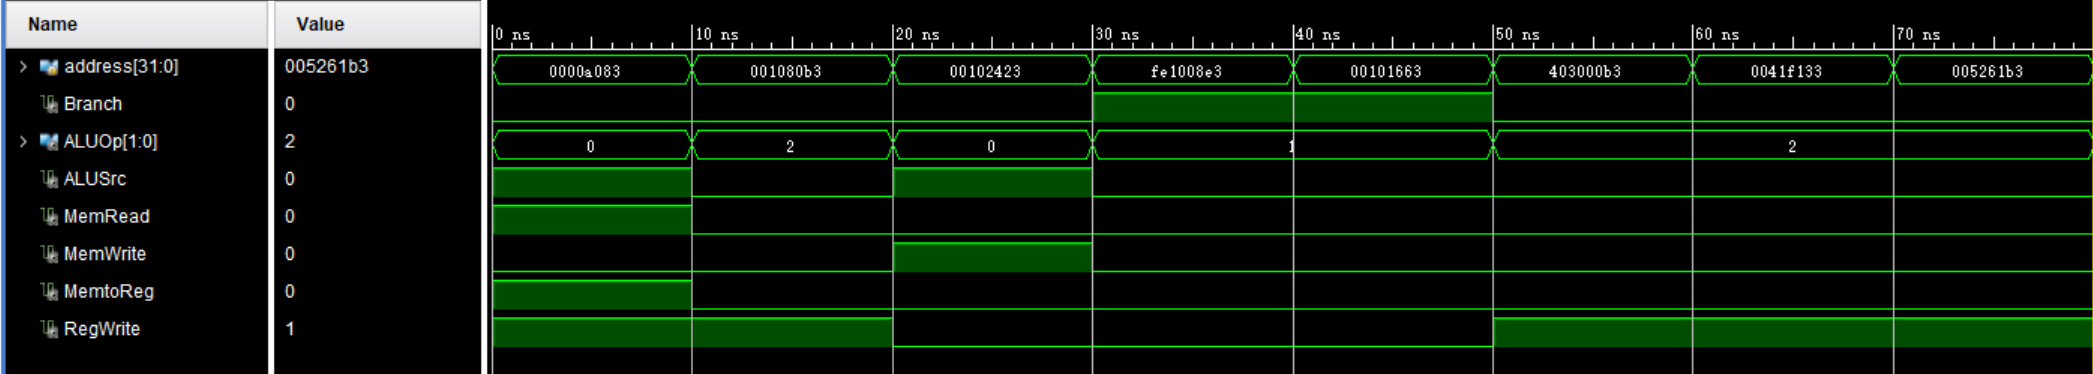
\includegraphics[width=\textwidth]{tb1.png}
    \caption{Controller Testbench}
\end{figure}

The instructions are from lab slides: \texttt{lw}, \texttt{add}, \texttt{sw}, \texttt{beq}, \texttt{bne}, \texttt{sub}, \texttt{and}, \texttt{or}.

\section*{ALU}

\subsection*{Code}

\begin{center}
    \begin{minted}{verilog}
module ALU(
input [31:0] Inst,
input [31:0] Read_data_1,
input [31:0] Read_data_2,
input [31:0] Imme,
input [1:0] ALUOp,
input ALUSrc,
output reg [31:0] ALU_result,
output Zero
    );

wire [3:0] ALUControl;
wire [31:0] Operand2;

ALU_Control ALU_Control(
.ALUOp(ALUOp),
.Inst(Inst),
.ALUControl(ALUControl)
);

assign Operand2 = ALUSrc ? Imme : Read_data_2;
assign Zero = ALU_result == 0;

always @* begin
    case(ALUControl)
        4'b0000:
        begin
            ALU_result = Read_data_1 & Operand2;
        end
        4'b0001:
        begin
            ALU_result = Read_data_1 | Operand2;
        end
        4'b0010:
        begin
            ALU_result = Read_data_1 + Operand2;
        end
        4'b0110:
        begin
            ALU_result = Read_data_1 - Operand2;
        end
    endcase
end
endmodule

module ALU_Control(
input [1:0] ALUOp,
input [31:0] Inst,
output reg [3:0] ALUControl
    );

wire [6:0] funct7;
wire [2:0] funct3;
assign funct7 = Inst[31:25];
assign funct3 = Inst[14:12];

always @* begin
    case(ALUOp)
        2'b00: 
        begin
            ALUControl = 4'b0010;
        end
        2'b01:
        begin
            ALUControl = 4'b0110;
        end
        2'b10:
        begin
            case(funct7)
                7'b0000000:
                begin
                    case(funct3)
                        3'b000:
                        begin
                            ALUControl = 4'b0010;
                        end
                        3'b111:
                        begin
                            ALUControl = 4'b0000;
                        end
                        3'b110:
                        begin
                            ALUControl = 4'b0001;
                        end
                    endcase
                end
                7'b0100000:
                begin
                    ALUControl = 4'b0110;
                end
            endcase
        end
    endcase
end
endmodule
    \end{minted}
\end{center}

\subsection*{Testbench}

\begin{figure}[H]
    \centering
    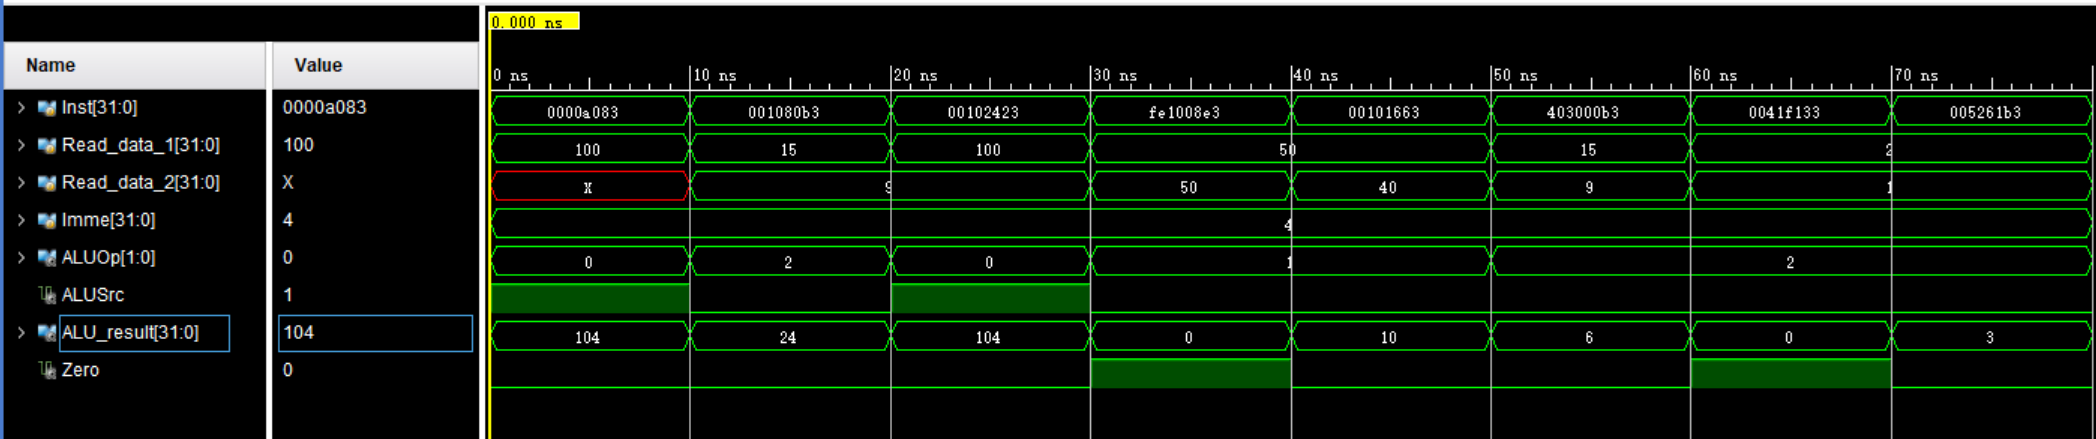
\includegraphics[width=\textwidth]{tb2.png}
    \caption{ALU Testbench}
\end{figure}

The instructions are the same as the previous testbench.
\end{document}